\section{Simulation}
To have a fair comparison, we decided to test 3 community detection methods: Newman modularity, InfoMap and Asymptotical surprise. In order to do it, we simulated rs-fMRI time-series and varied several parameters. We artificially created 300 nodes (brain voxels) which mimicked specific patterns of resting-state activation. 

We used the R package “neuRosim” to simulate the BOLD signal in each area ~\cite{Welvaert2011}. We manipulated the number of subjects (sample size) as well as the signal-to-noise ratio (SNR). For all the simulations, the baseline value of the time-series was set to 100~\cite{Welvaert2013}.

Two steps were necessary in order to get from the binary matrix representing the powerlaw ring of clique correlation to the generated time series representing the network. First, to ensure that the binary matrix of the simulated network  could be assimilated to a real correlation matrix, we computed from it the nearest (in Frobenius norm) Symmetric Positive Definite matrix (for more information see~\cite{Higham1988}).

The property of this matrix, allowed us to apply the Cholesky decomposition~\cite{Pourahmadi1999} on it.
The idea is that if $C$ is a correlation matrix , its Cholesky decomposition is defined as:
\begin{equation}
LL^T=C
\end{equation}
which allow the generation of correlated random variables as
\begin{equation}
LX=Y
\end{equation}
where $X$ are uncorrelated values (original simulated signal) and $Y$ correlated values (final simulated signal). 

Rician noise was added to the simulated time-series, independently for each subject and area. The simulated data neither included any slow drift component nor simulated physiological noise, nor spatial noise. The average SNR was defined as:

\begin{equation}
SNR=\frac{\bar{S}}{\sigma_N}
\end{equation}
With $\bar{S}$= the average magnitude of the signal; and $\sigma_N$= the standard deviation of the noise~\cite{Kruger2011}.


In the set of simulations, we varied both SNR and the number of subjects. The sample size was set equal to 1, 20, 40 ,60 ,80 subjects and the SNR ranged between 1 and none. 
After creating for each subject the 300 times series, a correlation matrix was computed expressing the relation between each pair of time series. Finally, to be able to realize a group analysis, these matrices were then z-transform and average. After thresholding it using the giant component threshold~\cite{Goerdt2001}, we ran on it the three community detection: Newman, InfoMap and asymptotic surprise.
Each simulation condition was repeated 27 times. 

We measured the validity of the output using different measures: the accuracy, sensitivity and specificity (see supplementary materials for Normalized Mutual Information (NMI) and Matthews correlation coefficient (Mcc) results). \\
\textcolor{red}{Explanation of why these coefficient here or not here???}

 These coefficients quantify the performance of a classification by comparing the “true” versus the “observed” classification. 
 Specifically, the accuracy which represents the proportion of true results is defined as

   \begin{equation}
   Accuracy= \frac{TP+TN}{TP+FP+FN+TN}
   \end{equation}
   
With $TP$ corresponding to the number of true positive, $TN$ of true negative, $FP$ of false positive, and $FN$ of false negative (misses).
With the same parameters, we also extracted the sensitivity (also called true positive rate) and the specificity (true negative rate):
 \begin{equation}
 sensitivity=\frac{TP}{TP+FN}
 \end{equation}
  \begin{equation}
 specificity=\frac{TN}{TN+FP}
 \end{equation}

For each simulation, we obtained a vector containing the communities, each affecting a network number to each areas. For each community, we scored as a TP, areas rightly gathered together; FP number of nodes wrongly affected in the community ; FN number of nodes of the community assigned to another community and finally TN all the areas correctly classified as out of the community. 

\section{Results}
\subsection{Simulation}
To test the difference of performance of the three methods, we
manipulated two parameters and evaluated the efficiency  of  the  method’s  output.  The  performance  was assessed by comparing the detected communities with the original created communities. The
rightfulness of each simulation was quantified using the sensitivity, specificity and accuracy coefficient (see simulation methods section, for Mcc and NMI see supplementary material).
A simulations varied the number
of simulated “subjects” and the SNR. 

\begin{figure}
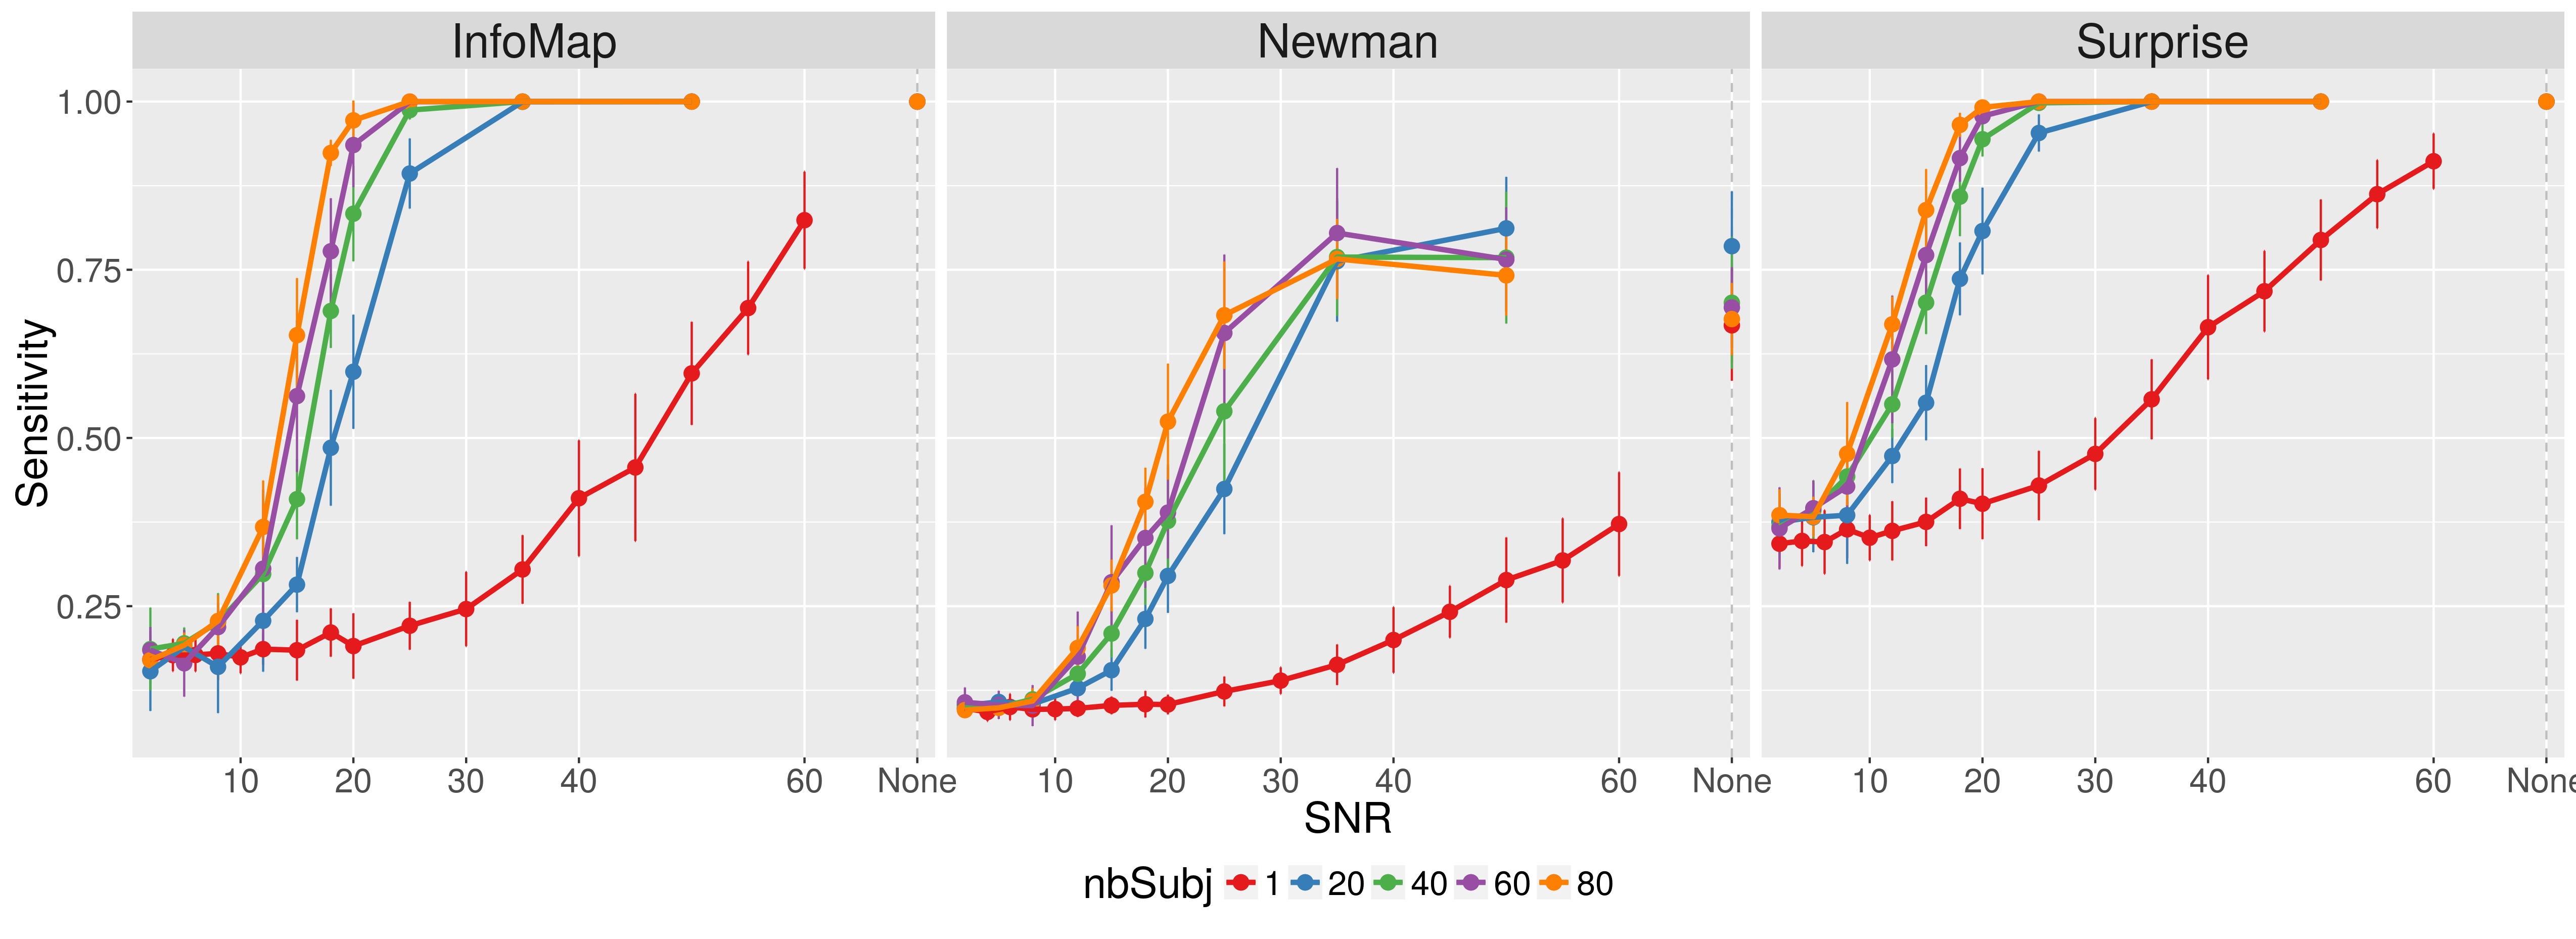
\includegraphics[width=0.9\textwidth]{images/Simu_Sensitivity_LFRClick_paper.png}\caption{blabla}
\label{FigSensitivity}

\end{figure}

Figure \ref{FigSensitivity} shows
for the three methods, the sensitivity coefficient variation depending of the sample size and
SNR. As expected, all methods, across sample sizes, increased their performance with increasing SNR. The Newman technique presents a lack of sensitivity even without any noise added, the maximum value is approximately 0.75. Asymptotical surprise and InfoMap display similar values for high SNR, with a "plateau" reaching a maximum sensitivity with a group sample bigger than 20 and with SNR above 30. However, with low SNR, asymptotical surprise presents a better sensitivity  with a value at approximately 0.35 against 0.2 for the InfoMap and 0.1 for Newman method.

The Specificity coefficient is equivalent across the three methods (see Figure \ref{FigSpecificity}). All display similar values with a quick convergence to the maximum value of 1 for high SNR and good performance (around 0.96) for low SNR. 


\begin{figure}[h!]
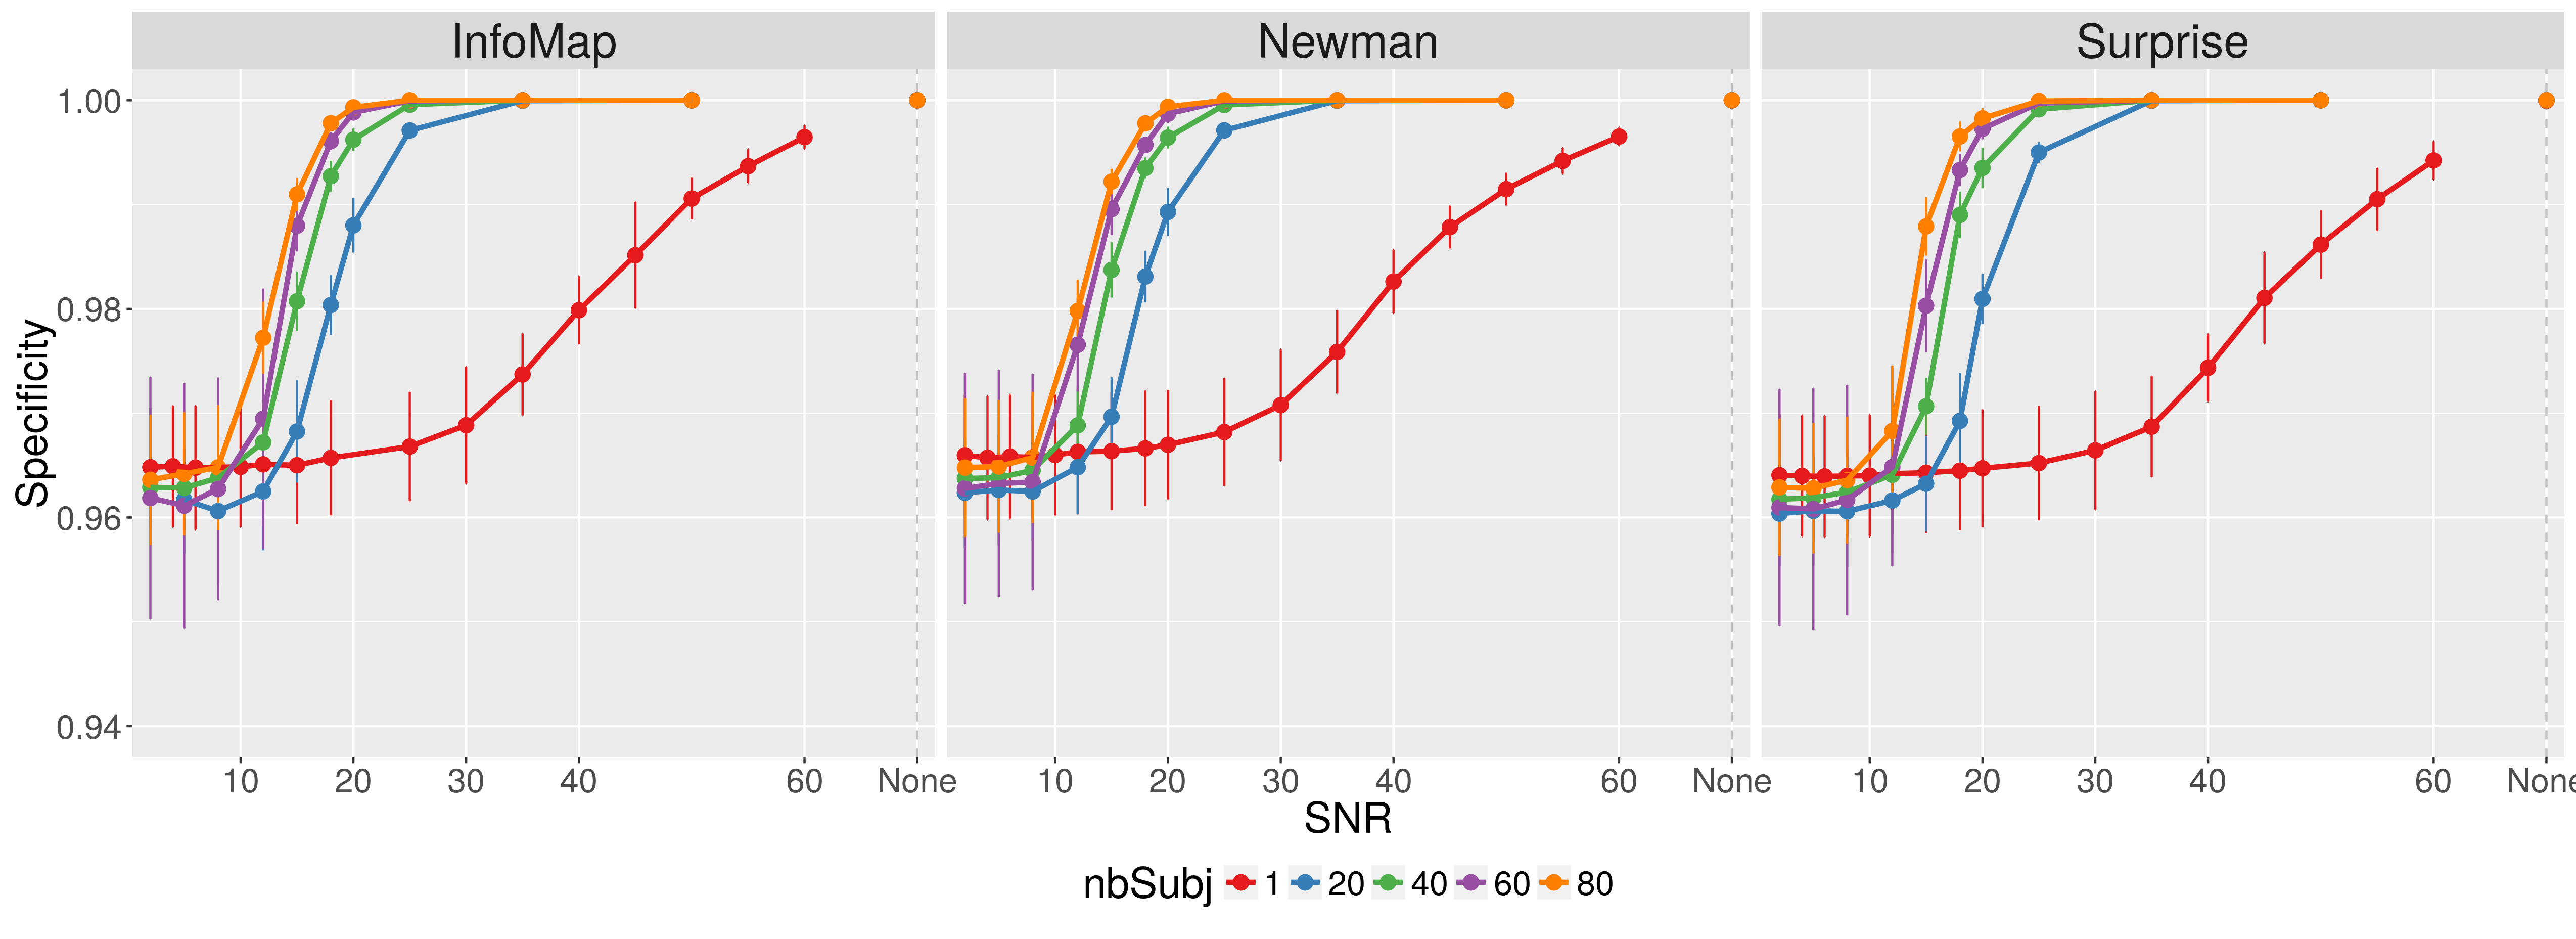
\includegraphics[width=0.9\textwidth]{images/Simu_Spec_LFRClick_paper.png}
\caption{blabla}
\label{FigSpecificity}

\end{figure}

Surprisingly, the accuracy coefficient reveal differences across the methods. Indeed, even if like expected they all converge to the maximum value with a SNR higher than 20, InfoMap exhibits a large variance specially when the SNR is low. Figure \ref{FigAccuracy} also displays the difference of slope to get to the plateau, between asymptotical surprise and the two others methods, due to a lower value of accuracy coefficient with low SNR for Newman and InfoMap.

In resume, unsurprisingly considering its resolution limit, Newman algorithm shows poor sensitivity. Indeed, its difficulty to detect small communities is increasing the number of community grouped together and so the number of nodes assigned wrongly (FN) which lower the sensitivity coefficient. 
More peculiar is the variance of the accuracy coefficient that InfoMap displays. After closer examination, it appears that for some of the simulation (4 simulations with 20 subjects: SNR=2, SNR=12 and 2 times SNR=8; 2 simulations with 60 subjects: SNR=8 and SNR=12; many times with simulation of 1 subject), InfoMap was unable to retrieve the right communities and instead was extracted only 2 which had as consequence to give an accuracy value close to 0 and so increase its variance.
Finally, the three methods are presenting strong and similar specificity values. 


\begin{figure}
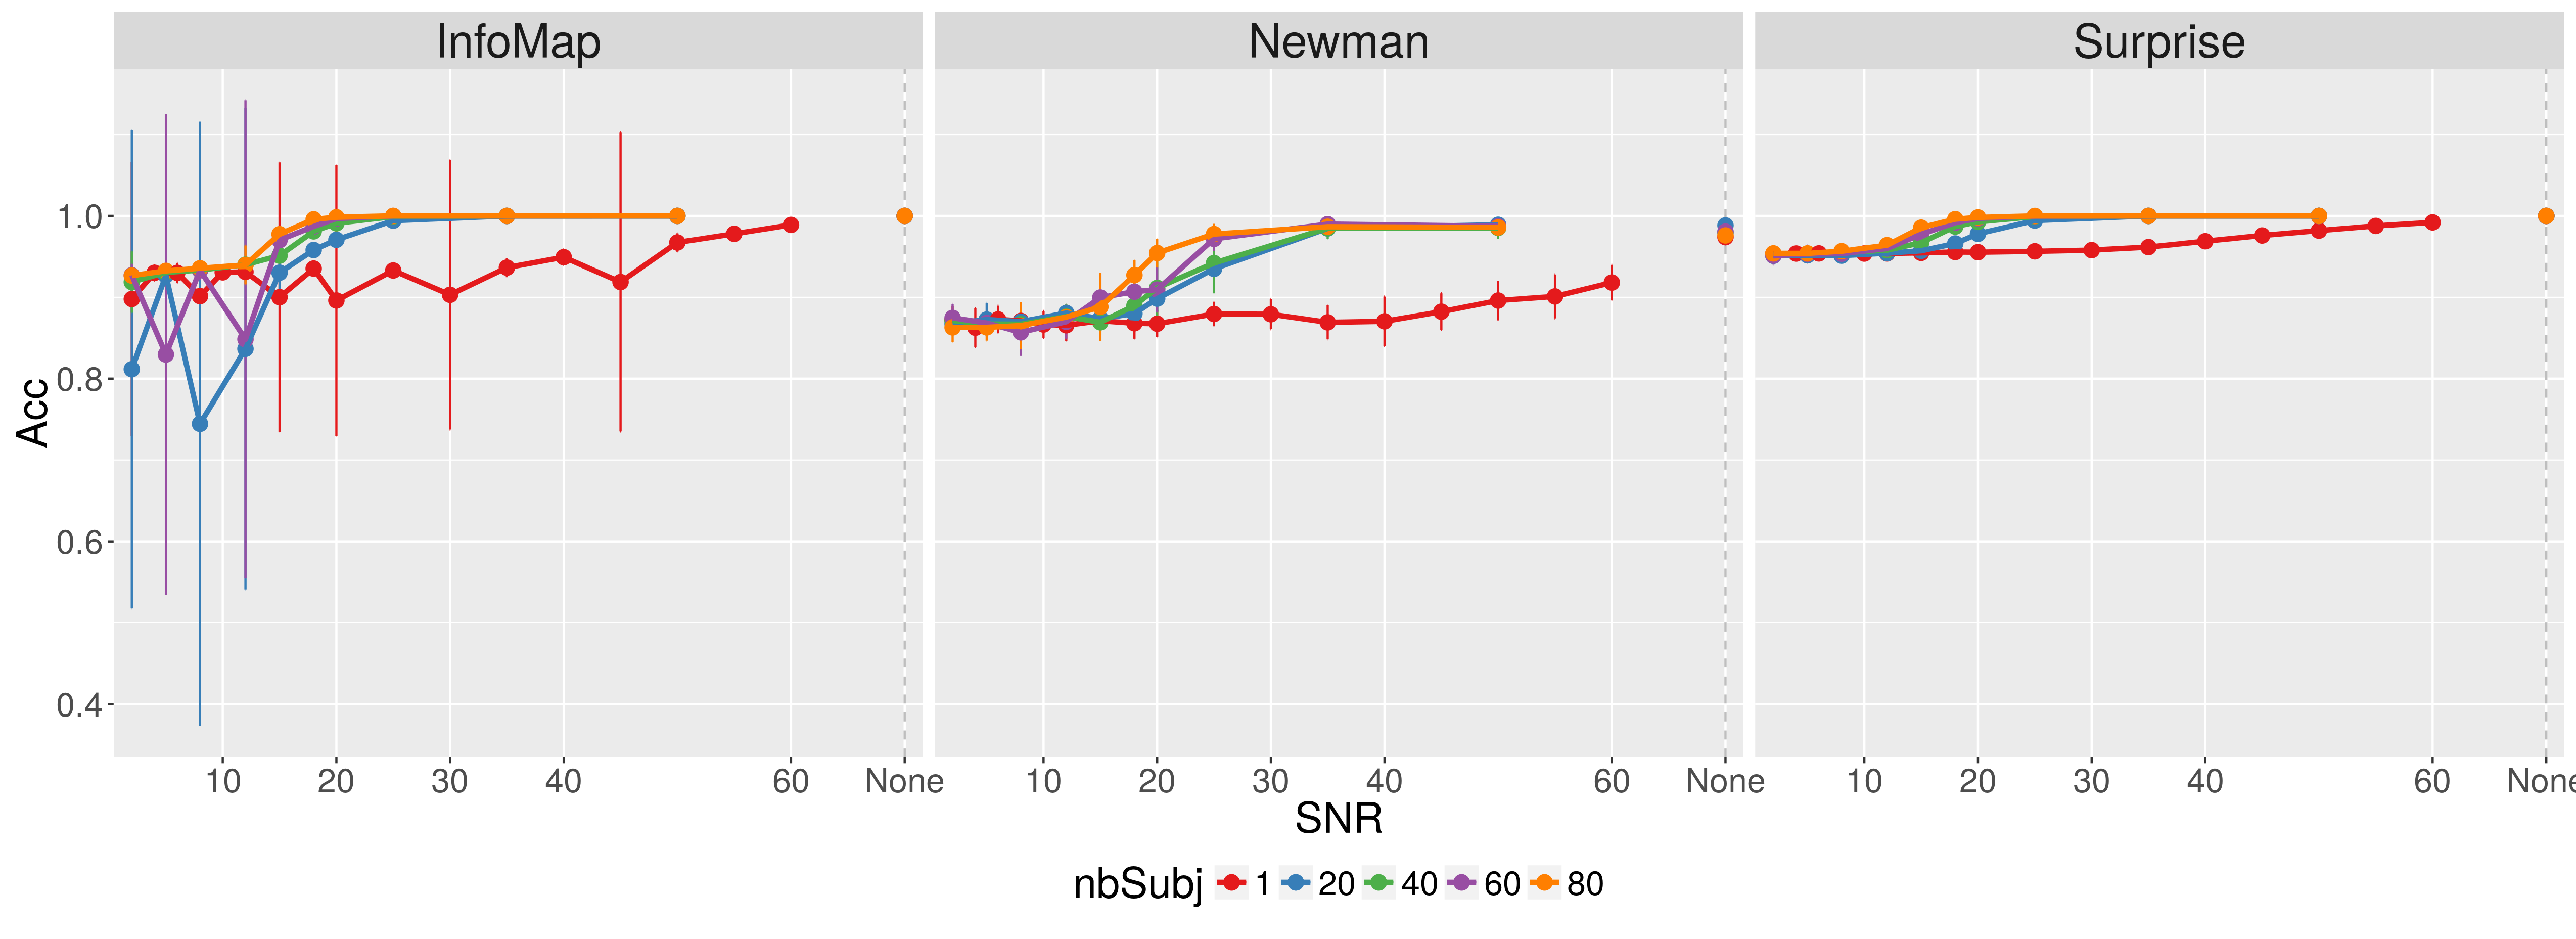
\includegraphics[width=0.9\textwidth]{images/Simu_Acc_LFRClick_paper.png}
\caption{blabla}
\label{FigAccuracy}
\end{figure}